\documentclass{standalone}

% graphics
\usepackage{tikz}
\usepackage{pgfplots}
\usepackage{siunitx}

\begin{document}

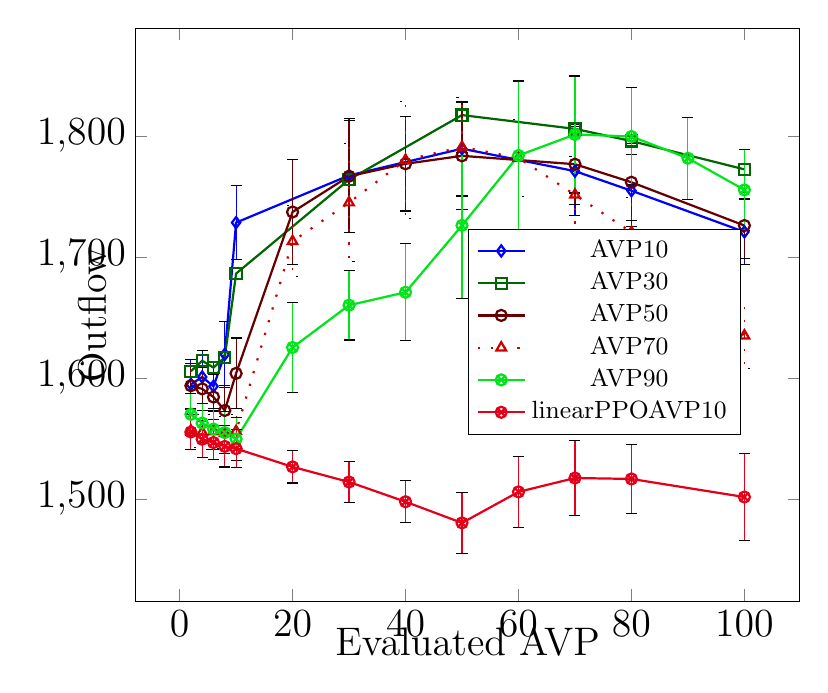
\begin{tikzpicture}[scale=1]
  \pgfplotsset{
      scale only axis,
      every x tick label/.append style={font=\Large},
      every y tick label/.append style={font=\Large},
	legend style={at={(0.5,0.65)},anchor=north west}
  }

\begin{axis}[
    legend style={font=\small},
	ylabel={\Large Outflow},
	x label style={at={(axis description cs:0.5,-0.03)},anchor=north},
	y label style={at={(axis description cs:-0.030,0.5)}, anchor=south},
	xlabel={\Large Evaluated AVP},
]

% trained on avp=10 
% dashdotdotted,
\addplot[mark=diamond, thick, mark options={solid, fill=blue!40, mark size=2 pt}, draw=blue, error bars/.cd, y dir=both, y explicit] table [x=a, y=b, y error=c] {
a	b   	c
2	1594.73	20.77
4 	1600.78 21.92	
6	1593.11 20.44
8	1619.46 27.24
10	1728.32 30.39
30 	1767.28 46.92
50	1789.38 39.06
70	1770.84 36.94
80	1754.68 29.82
100	1720.66 27.16
};
\label{AVP10}

% trained on avp=30
% error bars/.cd, y dir=both, y explicit,
\addplot[mark=square, thick, mark options={solid, fill=green!60, mark size=2 pt}, draw=black!60!green] table [x=a, y=b] {
a	b   	c
2	1605.56 17.93
4	1614.17 19.10
6	1608.55 21.58
8	1617.05 24.38
10	1686.20 32.29
30 	1763.86 49.79
50	1817.14 47.49
70	1805.76 34.11
80	1795.68 35.20
100	1772.32 30.88 
};
\label{AVP30}  

%densely dashed, 
\addplot[mark=o, thick, mark options={solid, fill=black!60!red, mark size=2pt}, draw=black!60!red, error bars/.cd, y dir=both, y explicit] table [x=a, y=b, y error=c] {
a	b   	c
2 1593.58 18.55
4 1590.95 17.89
6 1584.22 18.33
8 1573.13 20.52
10 1603.76 29.24
20 1737.07 43.04
30 1766.63 46.17
40 1776.89 38.99
50 1783.48 44.51
70 1776.56 33.09
80 1761.66 31.89
100 1725.91 27.05
};
\label{AVP50}

%densely dashed, 
\addplot[mark=triangle, thick, loosely dotted, mark options={solid, fill=red!60, mark size=2pt}, draw=black!20!red, error bars/.cd, y dir=both, y explicit] table [x=a, y=b, y error=c] {
a	b   	c
2 1556.35 13.87
4 1555.09 14.48
6 1555.81 14.30
8 1554.41 13.69
10 1555.92 14.15
20 1712.88 29.32
30 1744.85 48.62
40 1779.95 48.13
50 1790.78 40.98
60 1781.71 31.78
70 1751.29 31.96
80 1720.37 28.86
100 1634.90 26.76
};
\label{AVP70}

%densely dashed, 
\addplot[mark=otimes, thick, mark options={solid, fill=red!60, mark size=2pt},
draw=blue!10!green, error bars/.cd, y dir=both, y explicit] table [x=a, y=b, y error=c] {
a	b   	c
2 1569.96 17.40
4 1562.72 16.34
6 1557.79 16.67
8 1554.84 17.28
10 1549.51 17.87
20 1625.15 37.19
30 1660.07 28.71
40 1670.76 40.16
50 1725.98 60.36
60 1783.76 61.53
70 1801.12 48.34
80 1799.46 40.11
90 1781.50 33.85
100 1755.36 33.55
};
\label{AVP90}


%\addplot[mark=none, black, samples=2] {936.90};\label{Baseline}
%densely dashed, 
\addplot[mark=otimes, thick, mark options={solid, fill=blue!60, mark size=2pt},
draw=blue!10!red, error bars/.cd, y dir=both, y explicit] table [x=a, y=b, y error=c] {
a	b   	c
2 1555.34 14.31
4 1549.33 15.07
6 1546.63 13.90
8 1543.46 17.07
10 1541.63 15.80
20 1526.54 13.30
30 1514.05 16.60
40 1497.74 17.34
50 1480.25 25.14
60 1505.88 29.33
70 1517.33 30.85
80 1516.57 28.51
100 1501.63 36.18
};
\label{linearPPO}


\addlegendimage{/pgfplots/refstyle=AVP10}
\addlegendentry{AVP10}

\addlegendimage{/pgfplots/refstyle=AVP30}
\addlegendentry{AVP30}

\addlegendimage{/pgfplots/refstyle=AVP50}
\addlegendentry{AVP50}

\addlegendimage{/pgfplots/refstyle=AVP70}
\addlegendentry{AVP70}

\addlegendimage{/pgfplots/refstyle=AVP90}
\addlegendentry{AVP90}

\addlegendimage{/pgfplots/refstyle=linearPPO}
\addlegendentry{linearPPOAVP10}


%\addlegendimage{/pgfplots/refstyle=Baseline}
%\addlegendentry{Human Baseline}




\end{axis}
\end{tikzpicture}

\end{document}

